\documentclass[
  bibliography=totoc,     % Literatur im Inhaltsverzeichnis
  captions=tableheading,  % Tabellenüberschriften
  titlepage=firstiscover, % Titelseite ist Deckblatt
]{scrartcl}

% Paket float verbessern
\usepackage{scrhack}

%csv Dateien einlesen
\usepackage{csvsimple}

% Warnung, falls nochmal kompiliert werden muss
\usepackage[aux]{rerunfilecheck}

% unverzichtbare Mathe-Befehle
\usepackage{amsmath}
% viele Mathe-Symbole
\usepackage{amssymb}
% Erweiterungen für amsmath
\usepackage{mathtools}

% Fonteinstellungen
\usepackage{fontspec}
% Latin Modern Fonts werden automatisch geladen
% Alternativ zum Beispiel:
%\setromanfont{Libertinus Serif}
%\setsansfont{Libertinus Sans}
%\setmonofont{Libertinus Mono}

% Wenn man andere Schriftarten gesetzt hat,
% sollte man das Seiten-Layout neu berechnen lassen
\recalctypearea{}

% deutsche Spracheinstellungen
\usepackage[main=ngerman]{babel}


\usepackage[
  math-style=ISO,    % ┐
  bold-style=ISO,    % │
  sans-style=italic, % │ ISO-Standard folgen
  nabla=upright,     % │
  partial=upright,   % ┘
  warnings-off={           % ┐
    mathtools-colon,       % │ unnötige Warnungen ausschalten
    mathtools-overbracket, % │
  },                       % ┘
]{unicode-math}

% traditionelle Fonts für Mathematik
\setmathfont{Latin Modern Math}
% Alternativ zum Beispiel:
%\setmathfont{Libertinus Math}

\setmathfont{XITS Math}[range={scr, bfscr}]
\setmathfont{XITS Math}[range={cal, bfcal}, StylisticSet=1]

% Zahlen und Einheiten
\usepackage[
  locale=DE,                   % deutsche Einstellungen
  separate-uncertainty=true,   % immer Fehler mit \pm
  per-mode=symbol-or-fraction, % / in inline math, fraction in display math
]{siunitx}

% chemische Formeln
\usepackage[
  version=4,
  math-greek=default, % ┐ mit unicode-math zusammenarbeiten
  text-greek=default, % ┘
]{mhchem}

% richtige Anführungszeichen
\usepackage[autostyle]{csquotes}

% schöne Brüche im Text
\usepackage{xfrac}

% Standardplatzierung für Floats einstellen
\usepackage{float}
\floatplacement{figure}{htbp}
\floatplacement{table}{htbp}

% Floats innerhalb einer Section halten
\usepackage[
  section, % Floats innerhalb der Section halten
  below,   % unterhalb der Section aber auf der selben Seite ist ok
]{placeins}

% Seite drehen für breite Tabellen: landscape Umgebung
\usepackage{pdflscape}

% Captions schöner machen.
\usepackage[
  labelfont=bf,        % Tabelle x: Abbildung y: ist jetzt fett
  font=small,          % Schrift etwas kleiner als Dokument
  width=0.9\textwidth, % maximale Breite einer Caption schmaler
]{caption}
% subfigure, subtable, subref
\usepackage{subcaption}

% Grafiken können eingebunden werden
\usepackage{graphicx}
% größere Variation von Dateinamen möglich
\usepackage{grffile}

% schöne Tabellen
\usepackage{booktabs}

% Verbesserungen am Schriftbild
\usepackage{microtype}

% Literaturverzeichnis
\usepackage[
  backend=biber,
]{biblatex}
% Quellendatenbank
\addbibresource{lit.bib}
\addbibresource{programme.bib}

% Hyperlinks im Dokument
\usepackage[
  german,
  unicode,        % Unicode in PDF-Attributen erlauben
  pdfusetitle,    % Titel, Autoren und Datum als PDF-Attribute
  pdfcreator={},  % ┐ PDF-Attribute säubern
  pdfproducer={}, % ┘
]{hyperref}
% erweiterte Bookmarks im PDF
\usepackage{bookmark}

% Trennung von Wörtern mit Strichen
\usepackage[shortcuts]{extdash}
\author{%
  Samuel Haefs\\%
  \href{mailto:samuel.haefs@tu-dortmund.de}{samuel.haefs@tu-dortmund.de}%
  \and%
  Max Koch\\%
  \href{mailto:max.koch@tu-dortmund.de}{max.koch@tu-dortmund.de}%
}
\publishers{TU Dortmund – Fakultät Physik}

\subject{802}
\title{Das Hooksche Gesetz}
\date{%
  Durchführung: 31.10.2019
  \hspace{3em}
  Abgabe: 05.11.2019
}

\begin{document}
\maketitle
\thispagestyle{empty}
\tableofcontents
\newpage

%\printbibliography{}
 \section{Versuchbeschreibung}
\begin{figure}
  \centering
  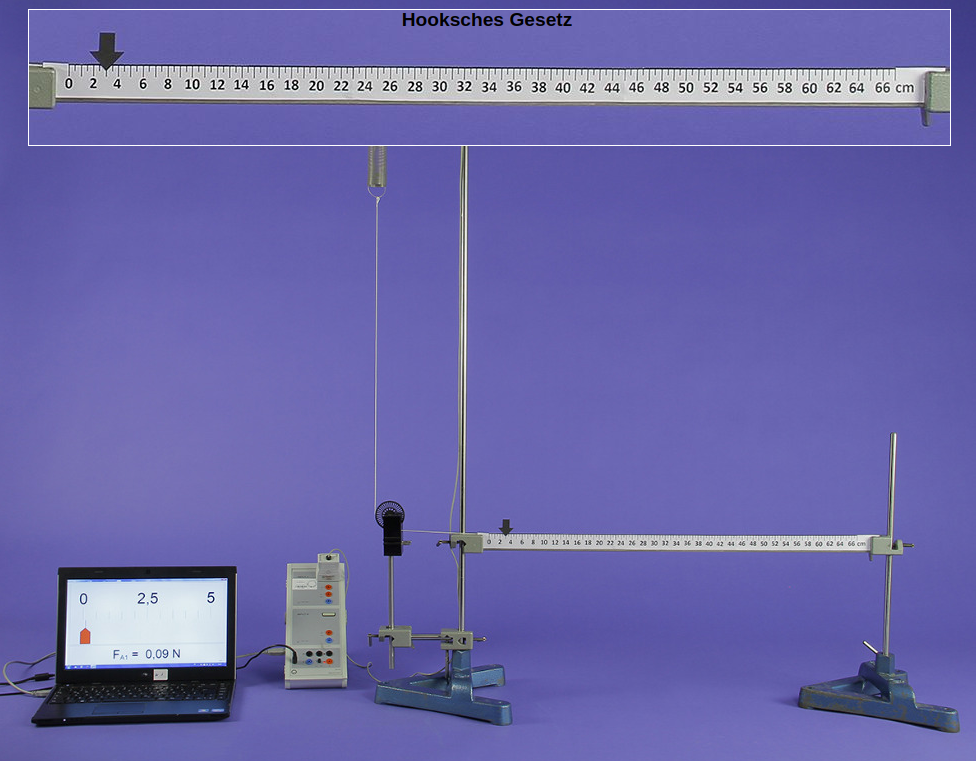
\includegraphics[width=\textwidth]{content/Hooksche_Gesetzt.png}
  \caption{Der Versuchsaufbau auf der \href{http://hyperion.didaktik.physik.uni-due.de/IBEs/Hooke.php}{Website}.}
  \label{fig:Versuchsaufbau}
\end{figure}
Im Versuch wird eine Feder an einem Kraftmesser angebracht. An dem losen Ende der Feder
wird dann ein Faden befestigt, der anschließend mit einer Rolle umgelenkt wird. 
Das andere Ende des Faden wird nun an einer Klammer befestigt,
die über ein Lineal beliebig verschiebar und fixierbar ist.
  \section{Versuchsdurchführung}
Zur Versuchsdurchführung wird die Klammer auf dem Lineal verschoben und anschließend fixiert.
Daraufhin wird der Wert auf dem Kraftmesser abgelesen und notiert.
Danach wird die Klammer wieder gelöst und erneut verschoben, bis die gewünschte Anzahl an Messwerten erreicht wird.
  \section{Versuchauswertung}
  \subsection{Mittlewertsbildung}
Durch die Durchfühnrung des Versuchs wurden folgende Werte gesammelt:
\begin{table}
  \centering
  \caption{Die Aufgenommen Daten}
  \label{tab:Messdaten}
  \begin{tabular}{c c}
  \toprule
  $ \Delta x \:/\: \si{\meter}$ & $F \:/\: \si{\newton}$ \\
  0.58 & 1.73 \\
  0.53 & 1.58 \\
  0.48 & 1.44 \\
  0.43 & 1.28 \\
  0.38 & 1.13 \\
  0.33 & 0.98 \\
  0.28 & 0.83 \\
  0.23 & 0.68 \\
  0.18 & 0.53 \\
  0.13 & 0.38 \\
  \bottomrule
  \end{tabular}
\end{table}
\FloatBarrier
Aus den aufgenommen Daten wurde nun der Mittelwert der Federkonstante $D$ wie folgt bestimmt
\begin{equation}
\sum_{i=1}^{10} \frac{1}{10} \cdot \frac{F_i}{\Delta x_i}
\end{equation}
Daraus ergibt sich
\begin{equation}
\bar{D} = 2.967234488336867
\end{equation}
Da dieser Wert nur der Mittelwert aller Federkonstante ist, ist er mit einer Unsicherheit behaftet.
Um die Unsicherheit $u$ zu berechnen, wird zunächst die Standardabweichung $\sigma$ berechnet.
\begin{equation}
\sigma = \sqrt{\frac{1}{9} \sum_{i=1}^{10} (D_i - \bar{D})^2}
\end{equation}
Daraus ergibt sich eine Standardabweichung von $\sigma = 0.02170138854644041
$
Damit lässt sich nun die Unsicherheit $u$ bestimmen
\begin{equation}
u = \frac{1}{ \sqrt{9}} \cdot \sigma
\end{equation}
Die errechnete Unsicherheit beträgt $u = 0.006862581619504244$

\subsection{lineare Ausgleichsrechnung}
\end{document}
